%% LyX 2.1.0 created this file.  For more info, see http://www.lyx.org/.
%% Do not edit unless you really know what you are doing.
\documentclass[12pt,letterpaper,english,12pt,english,openany,letterpaper,pagesize]{scrbook}
\usepackage[T1]{fontenc}
\usepackage[latin9]{inputenc}
\setlength{\parskip}{\medskipamount}
\setlength{\parindent}{0pt}
\usepackage{float}
\usepackage{textcomp}
\usepackage{amsthm}
\usepackage{amsmath}
\usepackage{graphicx}
\usepackage{setspace}
\onehalfspacing

\makeatletter

%%%%%%%%%%%%%%%%%%%%%%%%%%%%%% LyX specific LaTeX commands.
\pdfpageheight\paperheight
\pdfpagewidth\paperwidth

\newcommand{\lyxmathsym}[1]{\ifmmode\begingroup\def\b@ld{bold}
  \text{\ifx\math@version\b@ld\bfseries\fi#1}\endgroup\else#1\fi}

%% Because html converters don't know tabularnewline
\providecommand{\tabularnewline}{\\}

%%%%%%%%%%%%%%%%%%%%%%%%%%%%%% User specified LaTeX commands.
%\documentclass[12pt,spanish,fleqn,openany,letterpaper,pagesize]{scrbook}

%\usepackage[ansinew]{inputenc}
%\usepackage[spanish]{babel}
\usepackage{fancyhdr}
\usepackage{epsfig}
\usepackage{epic}
\usepackage{eepic}
\usepackage{amsmath}
\usepackage{threeparttable}
\usepackage{amscd}
\usepackage{here}
\usepackage{graphicx}
\usepackage{lscape}
\usepackage{tabularx}
\usepackage{subfigure}
\usepackage{longtable}


\usepackage{rotating} %Para rotar texto, objetos y tablas seite. No se ve en DVI solo en PS. Seite 328 Hundebuch
                        %se usa junto con \rotate, \sidewidestable ....


\renewcommand{\theequation}{\thechapter-\arabic{equation}}
\renewcommand{\thefigure}{\textbf{\thechapter-\arabic{figure}}}
\renewcommand{\thetable}{\textbf{\thechapter-\arabic{table}}}


\pagestyle{fancyplain}%\addtolength{\headwidth}{\marginparwidth}
\textheight22.5cm \topmargin0cm \textwidth16.5cm
\oddsidemargin0.5cm \evensidemargin-0.5cm%
\renewcommand{\chaptermark}[1]{\markboth{\thechapter\; #1}{}}
\renewcommand{\sectionmark}[1]{\markright{\thesection\; #1}}
\lhead[\fancyplain{}{\thepage}]{\fancyplain{}{\rightmark}}
\rhead[\fancyplain{}{\leftmark}]{\fancyplain{}{\thepage}}
\fancyfoot{}
\thispagestyle{fancy}%


\addtolength{\headwidth}{0cm}
\unitlength1mm %Define la unidad LE para Figuras
%\mathindent0cm %Define la distancia de las formulas al texto,  fleqn las descentra
\marginparwidth0cm
\parindent0cm %Define la distancia de la primera linea de un parrafo a la margen

%Para tablas,  redefine el backschlash en tablas donde se define la posici\'{o}n del texto en las
%casillas (con \centering \raggedright o \raggedleft)
\newcommand{\PreserveBackslash}[1]{\let\temp=\\#1\let\\=\temp}
\let\PBS=\PreserveBackslash

%Espacio entre lineas
\renewcommand{\baselinestretch}{1.1}

%Neuer Befehl f\"{u}r die Tabelle Eigenschaften der Aktivkohlen
\newcommand{\arr}[1]{\raisebox{1.5ex}[0cm][0cm]{#1}}

%Neue Kommandos
\usepackage{resources/Befehle}


%Trennungsliste
\hyphenation {Reaktor-ab-me-ssun-gen Gas-zu-sa-mmen-set-zung
Raum-gesch-win-dig-keit Durch-fluss Stick-stoff-gemisch
Ad-sorp-tions-tem-pe-ra-tur Klein-schmidt
Kohlen-stoff-Mole-kular-siebe Py-rolysat-aus-beu-te
Trans-port-vor-gan-ge}

%\pagenumbering{roman}
%\let\myTOC\tableofcontents
%\renewcommand\tableofcontents{%
%\myTOC
%\clearpage
%\pagenumbering{arabic}
%}

\makeatother

\usepackage{babel}
\begin{document}

\chapter{Mesh Editing with Laplacian Deform\label{sub:Laplacian-Deform}}

This work was accepted and completed for the software Blender \cite{blender}
that is an open source 3D application for modeling, animation, rendering,
compositing, video editing and game creation. In the Google Summer
of Code 2013 program which was administered for Google Inc.


\section{Synopsis}

The mesh editing is generally done with affine transformations, Blender3D
offers some tools to transform the vertices as \textquotedblleft proportional
editing object mode\textquotedblright{} with which the transformation
of some vertices is interpolated to the other vertices connected with
the use of simple distance functions.

This project proposes to implement a method for mesh editing based
on sketching lines defines by user and preserving the geometric details
of the surface.

This method captures the geometric details using a differential coordinates
representations. The differential coordinates captures the local geometric
information (curvature and direction) of the vertex based on its neighbors.
This method allows you to retrieve the best possible original model
after changing the positions of some vertices using the differential
coordinates of the original model.


\section{Benefits to Blender}

This project proposes a new tool for blender user that requires preserve
the geometric details of the surface during a modeling, transformation,
definition of the shape keys of the mesh vertices.

The method will allow novice users to edit any polygon mesh preserving
the surface details.

This method allows the user to define new shape keys in a most fast
and intuitive way.


\section{Deliverables}
\begin{itemize}
\item A new mesh editing tool for Blender. 
\item Some pages of documentation to be included in the manual 
\item A technical document for developers to improve the method in the future. 
\item A tutorial explaining the use of the tool.
\end{itemize}

\section{Project Details}

The project would divide into several parts:
\begin{enumerate}
\item Calculate the differential coordinates. 
\item Store the fixed vertices (Hard constraints). 
\item Store positions of the edited vertices. 
\item Store the more representative vertex for retrieve rotation of every
differential coordinate.
\item Solve the initial solution \textendash{} in least-squares sense. 
\item Rotate the differential coordinates with base on initial solution
and more representative vertex.
\item Reconstruct the surface \textendash{} in least-squares sense. 
\item Generation of the documentation and tutorials.
\end{enumerate}

\section{Project Schedule}
\begin{itemize}
\item 2 Weeks: Calculate the differential coordinates.
\item 2 Weeks: Store the fixed vertexes (Hard constraints).
\item 2 Weeks: Store positions of the edited vertexes.
\item 2 Weeks: Compute initial solution.
\item 2 Weeks: Rotate differential coordinates.
\item 2 Weeks: Reconstruct the surface \textendash{} in least-squares sense. 
\item 1 Weeks: Testing the tool and Define and implement graphical user
integration.
\item 2 Weeks: Generation of the documentation and tutorials.
\end{itemize}

\section{Laplacian Deform}

The Laplacian deform allows to pose a mesh while preserving geometric
details of the surface. This method allows to defines a set of anchor
vertices, and then moves some of them around. The system keeps the
rest of the anchor vertices in fixed positions, and calculates the
best possible locations of all the remaining vertices to preserve
the original geometric details.

This work adapt the method proposed by Sorkine \cite{Sorkine2004}
for mesh deformations, delete the use of static vertices and allow
application of this system in hybrid meshes composes by triangles
and quads with the TQLBO proposed.

This method captures the geometric details using a differential coordinates
representations. The differential coordinates captures the local geometric
information (curvature and direction) of the vertex based on its neighbors
how show in figure \ref{fig:DifferentialCoor}.

\begin{figure}[H]
\noindent \begin{centering}
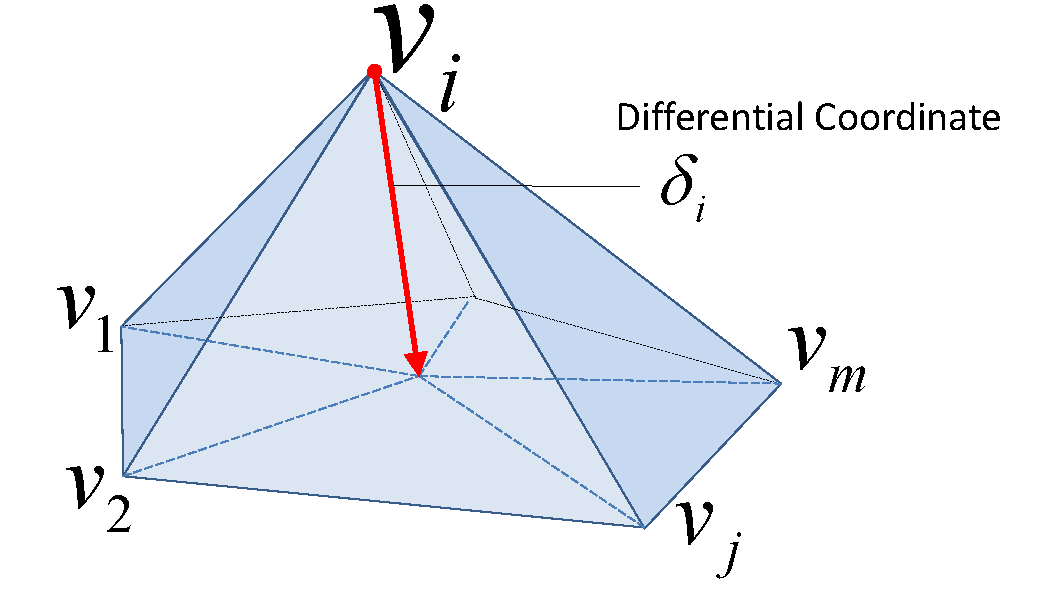
\includegraphics[width=0.7\columnwidth]{resources/figs/DifferentialCoordinates}
\par\end{centering}

\protect\caption{\label{fig:DifferentialCoor} Difference between $v_{i}$ and the
center of mass of its neighbors $v_{1},...,v$.}
\end{figure}


\begin{equation}
\delta_{i}=\overset{m}{\underset{j=1}{\sum}}w_{ij}\left(v_{i}-v_{j}\right)\label{eq:DifferentialCoordinate}
\end{equation}


Where $\delta_{i}$ is the differential coordinate for vertex $v_{i}$.
The $v_{j}$ are the immediate neighbors of $v_{i}$, and $w_{ij}$
is the weight between vertex $v_{i}$ and $v_{j}$ defined in equation
\ref{PAPER:eq:TQLBO_wij} that is TQLBO.

Then the linear systems for find the new pose of a mesh is.

\begin{equation}
\begin{bmatrix}w_{l}L\\
W_{c}
\end{bmatrix}X=\begin{bmatrix}\delta\\
W_{c}C
\end{bmatrix}\label{eq:LaplacianDefomSystem}
\end{equation}


Where $w_{l}$ is the weight for Laplacian Matrix $L$, the Laplacian
matrix $L$ was defined in equation \ref{PAPER:eq:TQLBO_Simple_Matrix}
. $Wc$ is a matrix that contains ones int the indexes of anchors
vertices. $C$ is a vector with coordinates of anchors vertices after
several transformations. $\delta$ are the differential coordinates
defined in equation \ref{eq:DifferentialCoordinate}.


\section{Performance Testing of Solvers }

For this project we choose a numerical solver to be included in Blender
software with base in a performance evaluation of computation of the
initial factorization of the Laplacian deform system.

Linear equation system to solve

\noindent \begin{center}
$\begin{bmatrix}w_{l}L\\
W_{c}
\end{bmatrix}X=\begin{bmatrix}\delta\\
W_{c}C
\end{bmatrix}$
\par\end{center}

Solving the sparse linear system

\noindent \begin{center}
$Ax=b$
\par\end{center}

Where:

\noindent \begin{center}
$A=\begin{bmatrix}w_{l}L\\
W_{c}
\end{bmatrix}$
\par\end{center}

\noindent \begin{center}
$x=V$
\par\end{center}

\noindent \begin{center}
$b=\begin{bmatrix}\delta\\
W_{c}C
\end{bmatrix}$
\par\end{center}


\subsection{Hardware Specification }
\begin{itemize}
\item Processor: AMD Quad-Core 2.40 GHz 
\item RAM: 8.0 GB 
\item OS: Windows 7 Professional 
\item Graphics controller: NVIDIA Quadro FX 570
\end{itemize}

\subsection{Software Specification }
\begin{description}
\item [{CGAL}] Computational Geometry Algorithms Library 
\item [{Graphite}] Research platform for computer graphics
\end{description}

\subsection{Numeric Solvers Used }
\begin{description}
\item [{CG:}] Conjugate gradient method. 
\item [{BICGSTAB:}] Biconjugate gradient stabilized method. 
\item [{GMRES:}] Generalized minimal residual method. 
\item [{SUPERLU:}] Sparse Direct Solver, LU decomposition with partial
pivoting. 
\item [{TAUCS\_LDLT:}] A library of sparse linear solvers with LDLT factorization. 
\item [{CHOLMOD:}] Supernodal sparse Cholesky factorization. 
\end{description}
LU factorization is a numerical method that works with large, sparse,
non-symmetric systems of linear equations \cite{Levy2005}. We choose
the implementation of LU factorization in a OpenNL-SuperLU library,
because this method show the better performance for the computation
of a solution for a Laplacian Deform linear system of equations presented
in equation \ref{eq:LaplacianDefomSystem} how see in the table and
plot \ref{tab:TimeVsSolvers}, \ref{fig:Plot-IniFactor}. OpenNL SuperLU
allow works with the Graphics Unit Processor GPU, for exploit the
capacity of GPU to work with parallel structures, more fast that traditional
CPU.

\begin{table}[H]
\begin{tabular}{|c|c|c|c|c|c|c|c|}
\hline 
Model & Vertices & CG & BICGSTAB & GMRES & SUPERLU & TAUCS & CHOLMOD\tabularnewline
\hline 
\hline 
Cross & 24 & 0.05 & 0.05 & 0.04 & 0.04 & 0.05 & 0.05\tabularnewline
\hline 
King & 538 & 0.83 & 0.63 & 0.71 & 0.61 & 0.68 & 0.79\tabularnewline
\hline 
YModel & 4770 & 19.60 & 16.44 & 16.93 & 16.06 & 16.88 & 17.95\tabularnewline
\hline 
Man & 10002 & 33.43 & 27.76 & 29.91 & 28.54 & 29.53 & 30.80\tabularnewline
\hline 
Neptune & 28052 & 133.97 & 136.46 & 136.39 & 133.21 & 142.87 & 142.76\tabularnewline
\hline 
Armadillo & 34594 & 194.48 & 174.88 & 175.80 & 169.92 & 181.70 & 183.49\tabularnewline
\hline 
\end{tabular}

\protect\caption{\label{tab:TimeVsSolvers}Vertices Vs Seconds, Laplacian Deform initial
factorization performance.}
\end{table}


\begin{figure}[H]
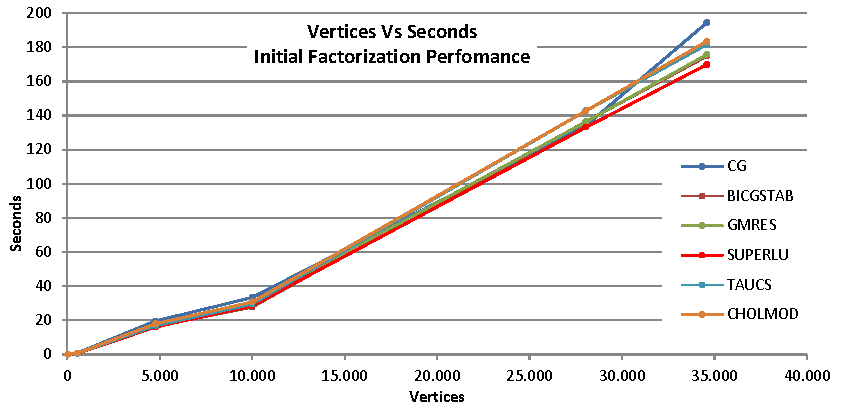
\includegraphics[width=1\textwidth]{Data/Benchmark}

\protect\caption{\label{fig:Plot-IniFactor}Plot of Vertices Vs Seconds, Initial factorization
performance.}
\end{figure}



\section{Results}

The user interface for software Blender can be seen in figure \eqref{fig:Panel-LaplacianDeform}.
In this tool the user define the anchor vertices with the use of vertex
groups a feature offered by Blender, the user configure this name
in the field \textsl{Anchors Vertex Group}. The \textsl{Bind} option
initiate the system and capture the geometry details in form of differential
coordinates and compute the factorization of the linear system, after
that the system is ready to repose meshes in real-time user interaction
session.

\noindent \begin{center}
\begin{figure}[H]
\noindent \begin{centering}
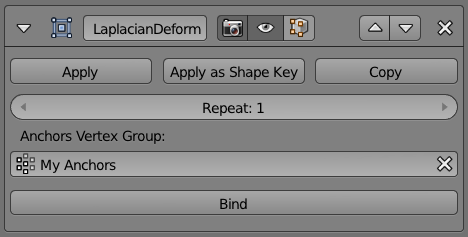
\includegraphics{resources/figs/Apinzonf_Diagram_Deform_Modifier_Panel_01}
\par\end{centering}

\protect\caption{\label{fig:Panel-LaplacianDeform}Panel inside blender user interface
of the Laplacian Deform modifier tool.}
\end{figure}

\par\end{center}

Figure \eqref{fig:Armadillo} shows the Laplacian Deform applied in
a model with 173K vertices, only anchor vertices was used and are
represented in blue color, when the user apply several transformation
(location, rotation, scale) over this anchors vertices, the system
find a solution and estimate the position of the vertices in yellow
color. This method work in real time, to achieve this the matrix $\begin{bmatrix}w_{l}L\\
W_{c}
\end{bmatrix}$ in the equation \eqref{eq:LaplacianDefomSystem} is decomposed in
matrix $LU$ with LU factorization only one time when the system initiate.
Once the matrix is factorized the system can solve the unknowns in
a fast way in term of milliseconds. For get better results the method
permits solve several times the system of equations, and not need
factorize matrix LU could be that at every iteration, only the differential
coordinates are adjust since the differential coordinates can be rotated
at every iteration and get better results. In the figure only four
iterations were used, but the system find good solutions with only
one iteration when the angle of rotations are less that $\pi$.

\begin{figure}[H]
\noindent \begin{centering}
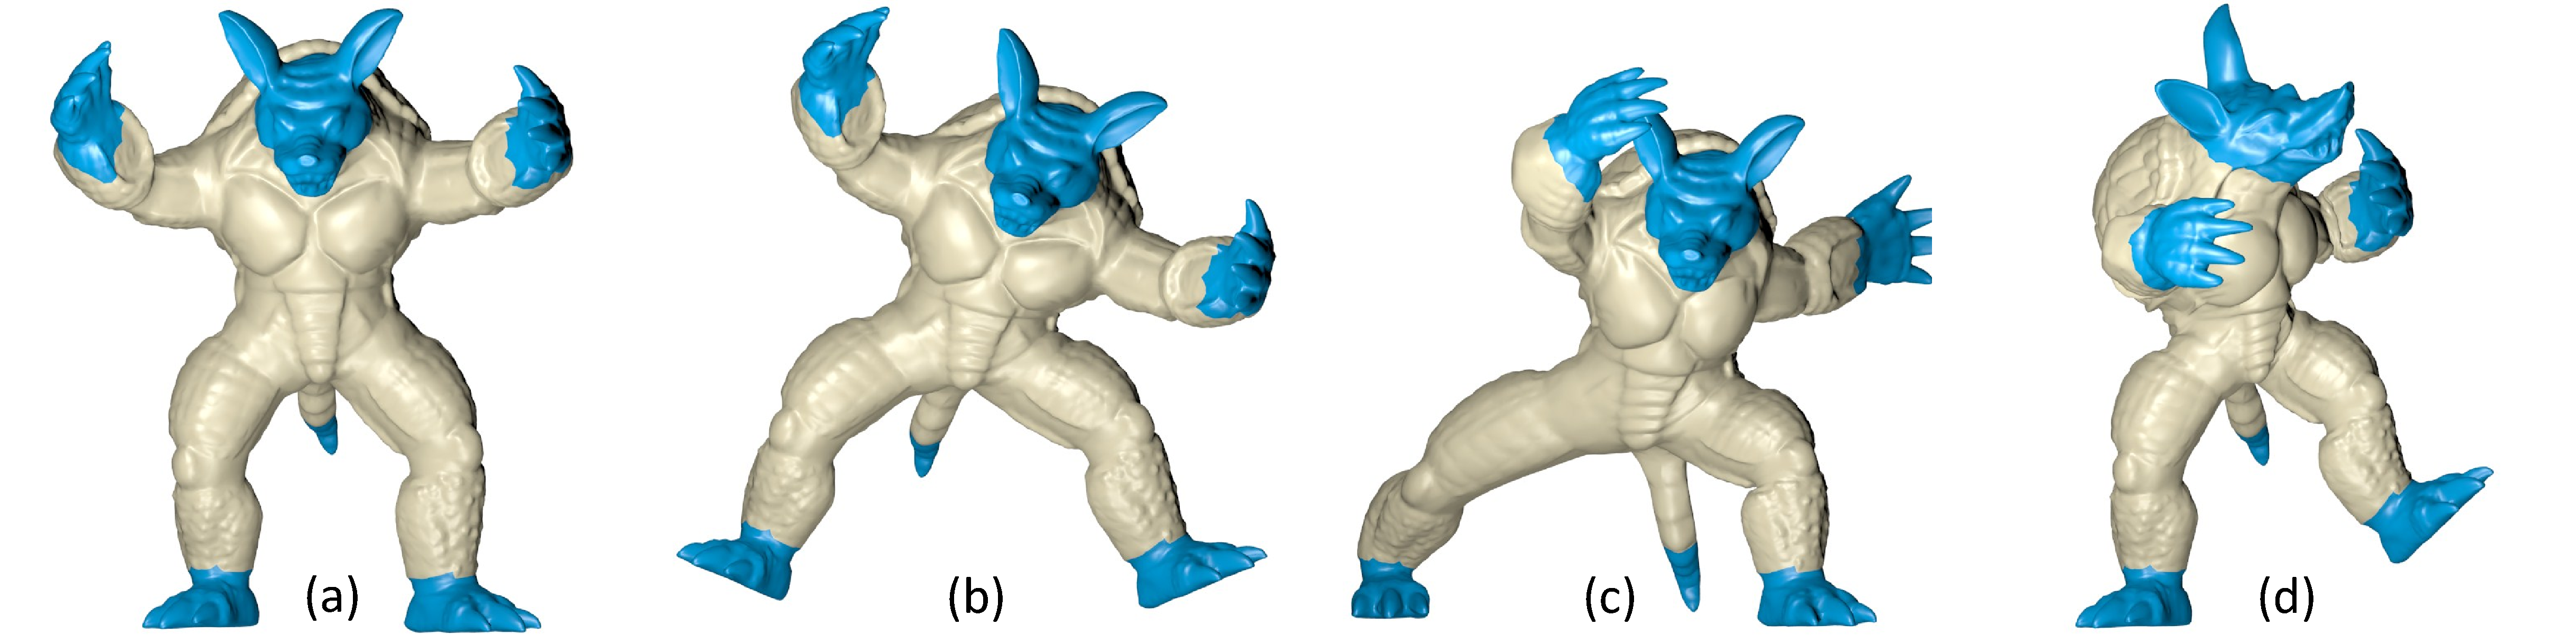
\includegraphics[width=1\textwidth]{resources/figs/Armadillo}
\par\end{centering}

\protect\caption{\label{fig:Armadillo}Anchor vertices in blue color. (a) Original
Model, (b,c,d) new poses change only anchor vertices, system find
positions for vertices in yellow color.}
\end{figure}


In figure \ref{fig:Cactus} show a comparison after made a one simple
transformation that consist in rotate $70\lyxmathsym{�}$ to right
the parts in blue color. between traditional method to interpolate
the changes made in some parts of the mesh to entire model. The results
for simple interpolation is show in \ref{fig:Cactus}.b and show how
the main trunk loss your shape and is rotated. The propagation of
changes made with Laplacian deform (figure \ref{fig:Cactus}.c) for
the same transformation show better results and how the details and
shape of the original model are preserve as best as possible.

\begin{figure}[H]
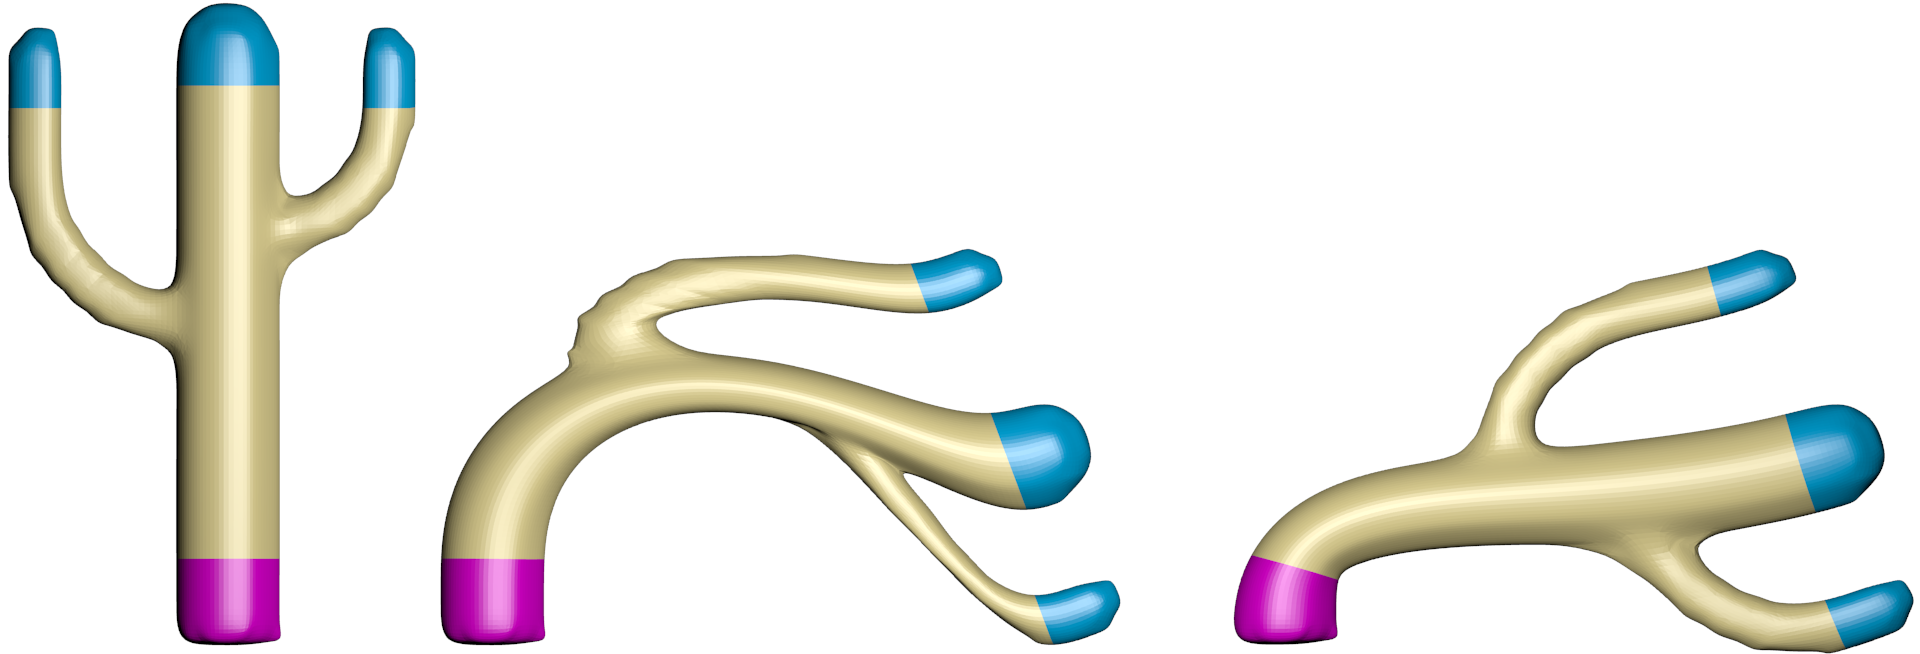
\includegraphics[width=1\textwidth]{resources/figs/cactus}

\protect\caption{\label{fig:Cactus}(a) Original cactus model. (b) Rotate 70� to right
the blue segments with basic interpolation (c) Rotate 70� to right
the blue segments with Laplacian deform tool.}
\end{figure}


The Laplacian Deform tool allow a user to repose a model while preserve
the geometry details in the figure \ref{fig:Horse}.b y \ref{fig:Horse}c
you can see the new pose of he horse after five transformations and
rotation of the head, in figure \ref{fig:Horse}.b you was use basic
interpolation and the shape and details are lost with every change
made. In figure \ref{fig:Horse}..c yo can see how the new pose of
the horse look more natural, and how the body and neck, of the horse
preserve the original shape, this comparison show that method allow
to apply any number of transformations without lost details, could
be the system try to recover geometry details with base in the original
pose of the model.

\begin{figure}[H]
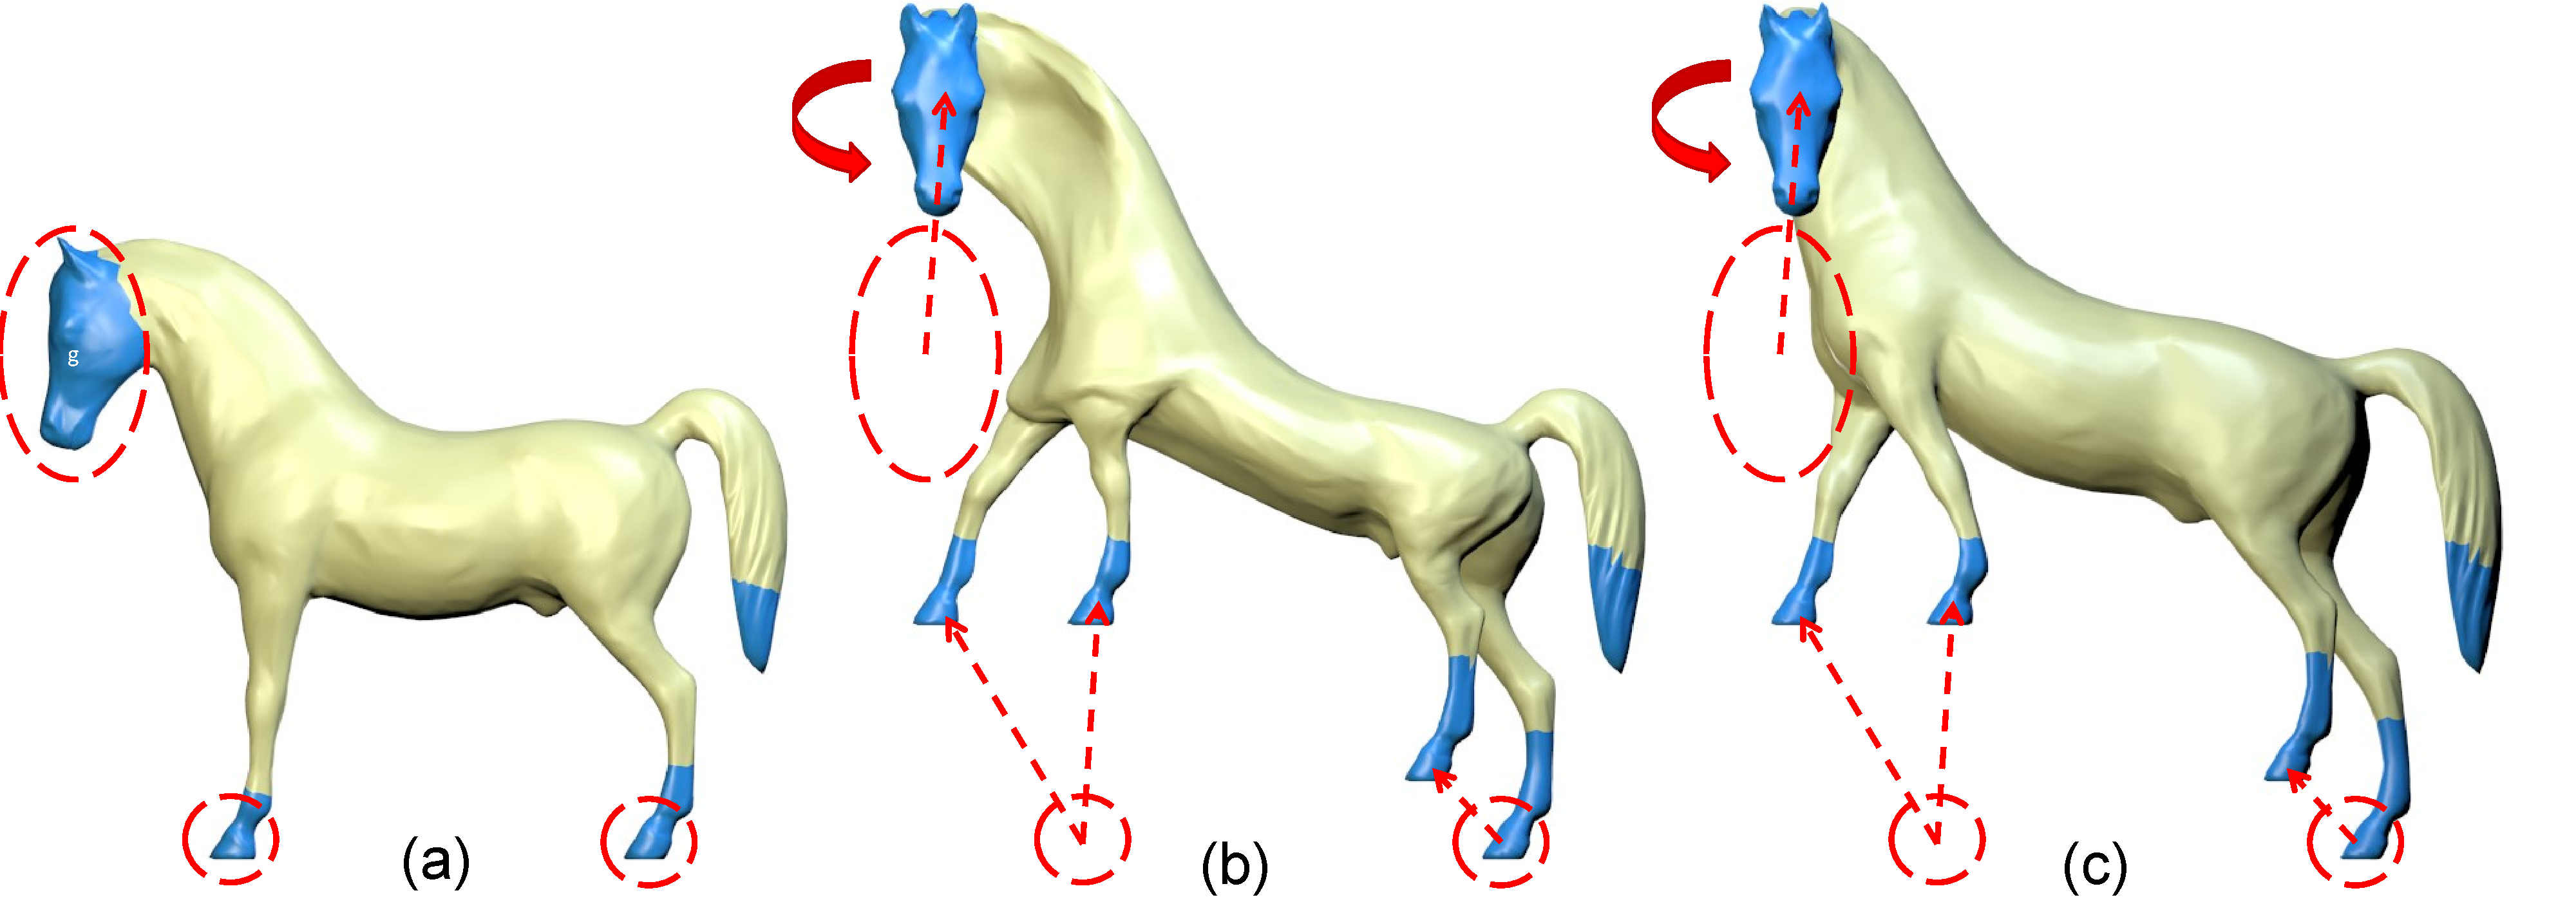
\includegraphics[width=1\textwidth]{resources/figs/horse}

\protect\caption{\label{fig:Horse}(a) Original Horse model. (b) Translate and rotate
the blue segments with basic interpolation (c) Translate and rotate
the blue segments with Laplacian deform tool.}
\end{figure}


\bibliographystyle{plain}
\addcontentsline{toc}{chapter}{\bibname}\bibliography{bibliografia/listado_inicial,TQLBO-paper/template,D:/src/blender/GSoC/GSOC2013/bibliography_mesh_editing,SIBGRAPI2013/template}

\end{document}
